%%%%%%%%%%%%%%%%%%%%%%%%%%%%%%%%%%%%%%%%%%%%%%%%%%%%%%%%%%%%%%%%%%%%%%%%%%%%%%%
% Short Sectioned Assignment LaTeX Template Version 1.0 (5/5/12)
% This template has been downloaded from: http://www.LaTeXTemplates.com
% Original author:  Frits Wenneker (http://www.howtotex.com)
% License: CC BY-NC-SA 3.0 (http://creativecommons.org/licenses/by-nc-sa/3.0/)
%%%%%%%%%%%%%%%%%%%%%%%%%%%%%%%%%%%%%%%%%%%%%%%%%%%%%%%%%%%%%%%%%%%%%%%%%%%%%%%

%\documentclass[paper=a4, fontsize=11pt]{scrartcl} % A4 paper and 11pt font size
\documentclass[11pt, a4paper]{book}
\usepackage[T1]{fontenc} % Use 8-bit encoding that has 256 glyphs
\usepackage[utf8]{inputenc}
\usepackage{fourier} % Use the Adobe Utopia font for the document - comment this line to return to the LaTeX default
\usepackage{listings} % para insertar código con formato similar al editor
\usepackage[spanish, es-tabla]{babel} % Selecciona el español para palabras introducidas automáticamente, p.ej. "septiembre" en la fecha y especifica que se use la palabra Tabla en vez de Cuadro
\usepackage{url} % ,href} %para incluir URLs e hipervínculos dentro del texto (aunque hay que instalar href)
\usepackage{graphics,graphicx, float} %para incluir imágenes y colocarlas
\usepackage[gen]{eurosym} %para incluir el símbolo del euro
\usepackage{cite} %para incluir citas del archivo <nombre>.bib
\usepackage{enumerate}
\usepackage{hyperref}
\usepackage{graphicx}
\usepackage{tabularx}
\usepackage{booktabs}

\setlength{\parindent}{0cm} % Anular sangría

\usepackage[table,xcdraw]{xcolor}
\hypersetup{
	colorlinks=true,	% false: boxed links; true: colored links
	linkcolor=black,	% color of internal links
	urlcolor=cyan		% color of external links
}
\renewcommand{\familydefault}{\sfdefault}
\usepackage{fancyhdr} % Custom headers and footers
\pagestyle{fancyplain} % Makes all pages in the document conform to the custom headers and footers
\fancyhead[L]{} % Empty left header
\fancyhead[C]{} % Empty center header
\fancyhead[R]{Antonio Priego Raya} % My name
\fancyfoot[L]{} % Empty left footer
\fancyfoot[C]{} % Empty center footer
\fancyfoot[R]{\thepage} % Page numbering for right footer
%\renewcommand{\headrulewidth}{0pt} % Remove header underlines
\renewcommand{\footrulewidth}{0pt} % Remove footer underlines
\setlength{\headheight}{1pt} % Customize the height of the header

\usepackage{titlesec, blindtext, color}
\definecolor{gray75}{gray}{0.75}
\newcommand{\hsp}{\hspace{20pt}}
\titleformat{\chapter}[hang]{\Huge\bfseries}{\thechapter\hsp\textcolor{gray75}{|}\hsp}{0pt}{\Huge\bfseries}
\setcounter{secnumdepth}{4}
\usepackage[Lenny]{fncychap}
\setlength{\topmargin}{-22pt}
\setlength{\footskip}{130pt}


% Sección definición estilo de código
\usepackage{color}
\definecolor{minegro}{rgb}{0.1,0.1,0.1}
\definecolor{migris}{rgb}{0.39,0.39,0.39}
\definecolor{miverde}{rgb}{0.05,0.75,0.65}
\definecolor{minaranja}{rgb}{1,0.41,0.05}
\definecolor{fondo}{rgb}{0.92,0.93,0.94}
\lstset {
	language         = C++,
	basicstyle       = \footnotesize\sffamily\color{minegro},
	backgroundcolor  = \color{fondo},
	commentstyle     = \color{migris},
	frame            = single,
	numbers          = left,
	numbersep        = 5pt,
    numberstyle      = \scriptsize\color{migris},
	keywordstyle     = \color{miverde},
	showspaces       = false,
	showstringspaces = false,
	stringstyle      = \color{minaranja},
	tabsize          = 2,
	xleftmargin      = 18pt,
    columns          = flexible
}


% Sección definición de márgenes de capítulos
\newenvironment{mimargen}[2]{
\begin{list}{}{
	\setlength{\topsep}{0pt}
	\setlength{\leftmargin}{#1}
	\setlength{\rightmargin}{#2}
	\setlength{\itemindent}{\parindent}
}
\item[]}{\end{list}}


% Comienzo de documento
\begin{document}


	% Plantilla portada UGR
	\begin{titlepage}
 
 
\newlength{\centeroffset}
\setlength{\centeroffset}{-0.5\oddsidemargin}
\addtolength{\centeroffset}{0.5\evensidemargin}
\thispagestyle{empty}

\noindent\hspace*{\centeroffset}\begin{minipage}{\textwidth}

\centering

\includegraphics[width=0.9\textwidth]{imagenes/logo_ugr_mod.jpg}\\[1.4cm]

\textsc{ \Large TRABAJO FIN DE GRADO\\[0.2cm]}
\textsc{ GRADO EN INGENIERÍA INFORMÁTICA}\\[1cm]
% Upper part of the page
% 
% Title
{\Huge\bfseries Dispositivo para detección de escritura mediante Deep Learning en
un sistema empotrado\\
}
\noindent\rule[-1ex]{\textwidth}{3pt}\\[3.5ex]
{\large\bfseries Deep Learning en sistemas empotrados: TinyML}
\end{minipage}

\vspace{1.1cm}
\noindent\hspace*{\centeroffset}\begin{minipage}{\textwidth}
\centering

\textbf{Autor}\\ {Antonio Priego Raya}\\[2ex]
\textbf{Directores}\\
{Jesús González Peñalver\\
Juan José Escobar Pérez}\\[1.0cm]

\includegraphics[width=0.3\textwidth]{imagenes/etsiit_logo.png}\\[0.1cm]
\textsc{Escuela Técnica Superior de Ingenierías Informática y de Telecomunicación}\\
\textsc{---}\\
Granada, Julio de 2022
\end{minipage}
%\addtolength{\textwidth}{\centeroffset}
%\vspace{\stretch{2}}
\end{titlepage}




	% Plantilla prefacio UGR
	\chapter*{}
%\thispagestyle{empty}
%\cleardoublepage

%\thispagestyle{empty}

\begin{titlepage}
 
 
\setlength{\centeroffset}{-0.5\oddsidemargin}
\addtolength{\centeroffset}{0.5\evensidemargin}
\thispagestyle{empty}

\noindent\hspace*{\centeroffset}\begin{minipage}{\textwidth}

\centering
%
\includegraphics[width=0.9\textwidth]{imagenes/logo_ugr.jpg}\\[1.4cm]

%\textsc{ \Large PROYECTO FIN DE CARRERA\\[0.2cm]}
%\textsc{ INGENIERÍA EN INFORMÁTICA}\\[1cm]
% Upper part of the page
% 

 \vspace{3.3cm}

%si el proyecto tiene logo poner aquí
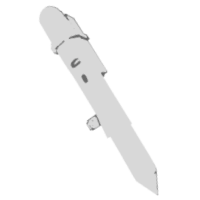
\includegraphics[width=0.25\textwidth]{imagenes/LogoSmartPen.png} 
 \vspace{0.5cm}

% Title

{\Huge\bfseries Dispositivo para detección de escritura mediante Deep Learning en
un sistema empotrado\\
}
\noindent\rule[-1ex]{\textwidth}{3pt}\\[3.5ex]
{\large\bfseries SmartPen\\[4cm]}
\end{minipage}

\vspace{2.5cm}
\noindent\hspace*{\centeroffset}\begin{minipage}{\textwidth}
\centering

\textbf{Autor}\\ {Antonio Priego Raya}\\[2.5ex]
\textbf{Directores}\\
{Juan José Escobar Pérez\\
Jesús González Peñalver}\\[2cm]
%
\includegraphics[width=0.15\textwidth]{imagenes/tstc.png}\\[0.1cm]
%\textsc{Departamento de Teoría de la Señal, Telemática y Comunicaciones}\\
%\textsc{---}\\
%Granada, mes de 201
\end{minipage}
%\addtolength{\textwidth}{\centeroffset}
\vspace{\stretch{2}}

 
\end{titlepage}






\cleardoublepage
\thispagestyle{empty}

\begin{center}
{\large\bfseries Detección de escritura mediante Deep Learning en
un sistema empotrado\\
}
\textsc{---}\\
{\small\bfseries Deep Learning en sistemas empotrados: TinyML.}\\
\end{center}
\begin{center}
Antonio Priego Raya\\
\end{center}

%\vspace{0.7cm}
\noindent{\textbf{Palabras clave}: TinyML, Machine learning, Deep learning,
Sistemas empotrados, Reconocimiento letras, Redes neuronales convolucionales,
...}\\

\vspace{0.7cm}
\noindent{\textbf{Resumen}}\\

\begin{comment}
Creación de un dispositivo autónomo con forma de lápiz en el que integrar un
sistema empotrado, concretamente haré uso de la Arduino Nano Sense 33 BLE.
El propósito de este dispositivo será la detección de letras en tiempo
real, registrando el movimiento del dispositivo para resolver la detección
de estas.\\
Para el procesamiento y clasificación de los movimientos se empleará
deep learning, con un modelo de red neuronal convolucional. Con la
particularidad de ejecutar el procesamiento del modelo en el propio
dispositivo, para dotarlo de autonomía.\\
Por tanto se desarrollarán todos los pasos propios del trabajo con
redes neuronales: diseño del modelo, recolección de datos, entrenamiento
del modelo, etc.\\
Complementario al dispositivo, también se creará un interfaz donde acceder
a las funciones del dispositivo.
\end{comment}
\cleardoublepage


\thispagestyle{empty}


\begin{center}
{\large\bfseries Project Title: Project Subtitle}\\
\end{center}
\begin{center}
First name, Family name (student)\\
\end{center}

%\vspace{0.7cm}
\noindent{\textbf{Keywords}: Keyword1, Keyword2, Keyword3, ....}\\

\vspace{0.7cm}
\noindent{\textbf{Abstract}}\\

Write here the abstract in English.

\chapter*{}
\thispagestyle{empty}

\noindent\rule[-1ex]{\textwidth}{2pt}\\[4.5ex]

Yo, \textbf{Antonio Priego Raya}, alumno de la titulación \textit{Grado en Ingeniería Informática}
de la \textbf{Escuela Técnica Superior
de Ingenierías Informática y de Telecomunicación de la Universidad de Granada}, con DNI 31033948W, autorizo la
ubicación de la siguiente copia de mi Trabajo Fin de Grado en la biblioteca del centro para que pueda ser
consultada por las personas que lo deseen.

\vspace{6cm}

\noindent Fdo: Antonio Priego Raya

\vspace{2cm}

\begin{flushright}
Granada a DÍA de Junio de 2022
\end{flushright}


\chapter*{}
\thispagestyle{empty}

\noindent\rule[-1ex]{\textwidth}{2pt}\\[4.5ex]

D. \textbf{Jesús González Peñalver}, Catedrático del departamento de Arquitectura y Tecnología de Computadores de la Universidad de Granada.

\vspace{0.5cm}

D. \textbf{Juan José Escobar Pérez}, Profesor Sustituto Interino del departamento de Arquitectura y Tecnología de Computadores de la Universidad de Granada.

\vspace{0.5cm}

\textbf{Informan:}

\vspace{0.5cm}

Que el presente trabajo, titulado \textit{\textbf{Dispositivo para detección de escritura mediante Deep Learning en
un sistema empotrado}},
ha sido realizado bajo su supervisión por \textbf{Antonio Priego Raya}, y autorizamos la defensa de dicho trabajo ante el tribunal
que corresponda.

\vspace{0.5cm}

Y para que conste, expiden y firman el presente informe en Granada a X de mes Julio de 2022.

\vspace{1cm}

\textbf{Los directores:}

\vspace{5cm}

\noindent \textbf{Jesús González Peñalver \ \ \ \ \ \ \ \ \ \ \ Juan José Escobar Pérez}

\chapter*{Agradecimientos}
\thispagestyle{empty}

       \vspace{1cm}


Poner aquí agradecimientos...



	
	% Índice de contenidos
	\newpage
	\tableofcontents

	% Índice de imágenes y tablas
	\newpage
	\listoffigures

	% Si hay suficientes se incluirá dicho índice
	\listoftables 
	\newpage

	% Diseño interfaz de usuario 
	\chapter{Interfaz de usuario}

En primer lugar, hice un diseño aproximado para la interfaz de usuario que
necesitaba haciendo uso de \textbf{\textit{QT Design Studio}}. Obteniendo el
siguiente resultado:

\begin{figure}[h]
    \centering
    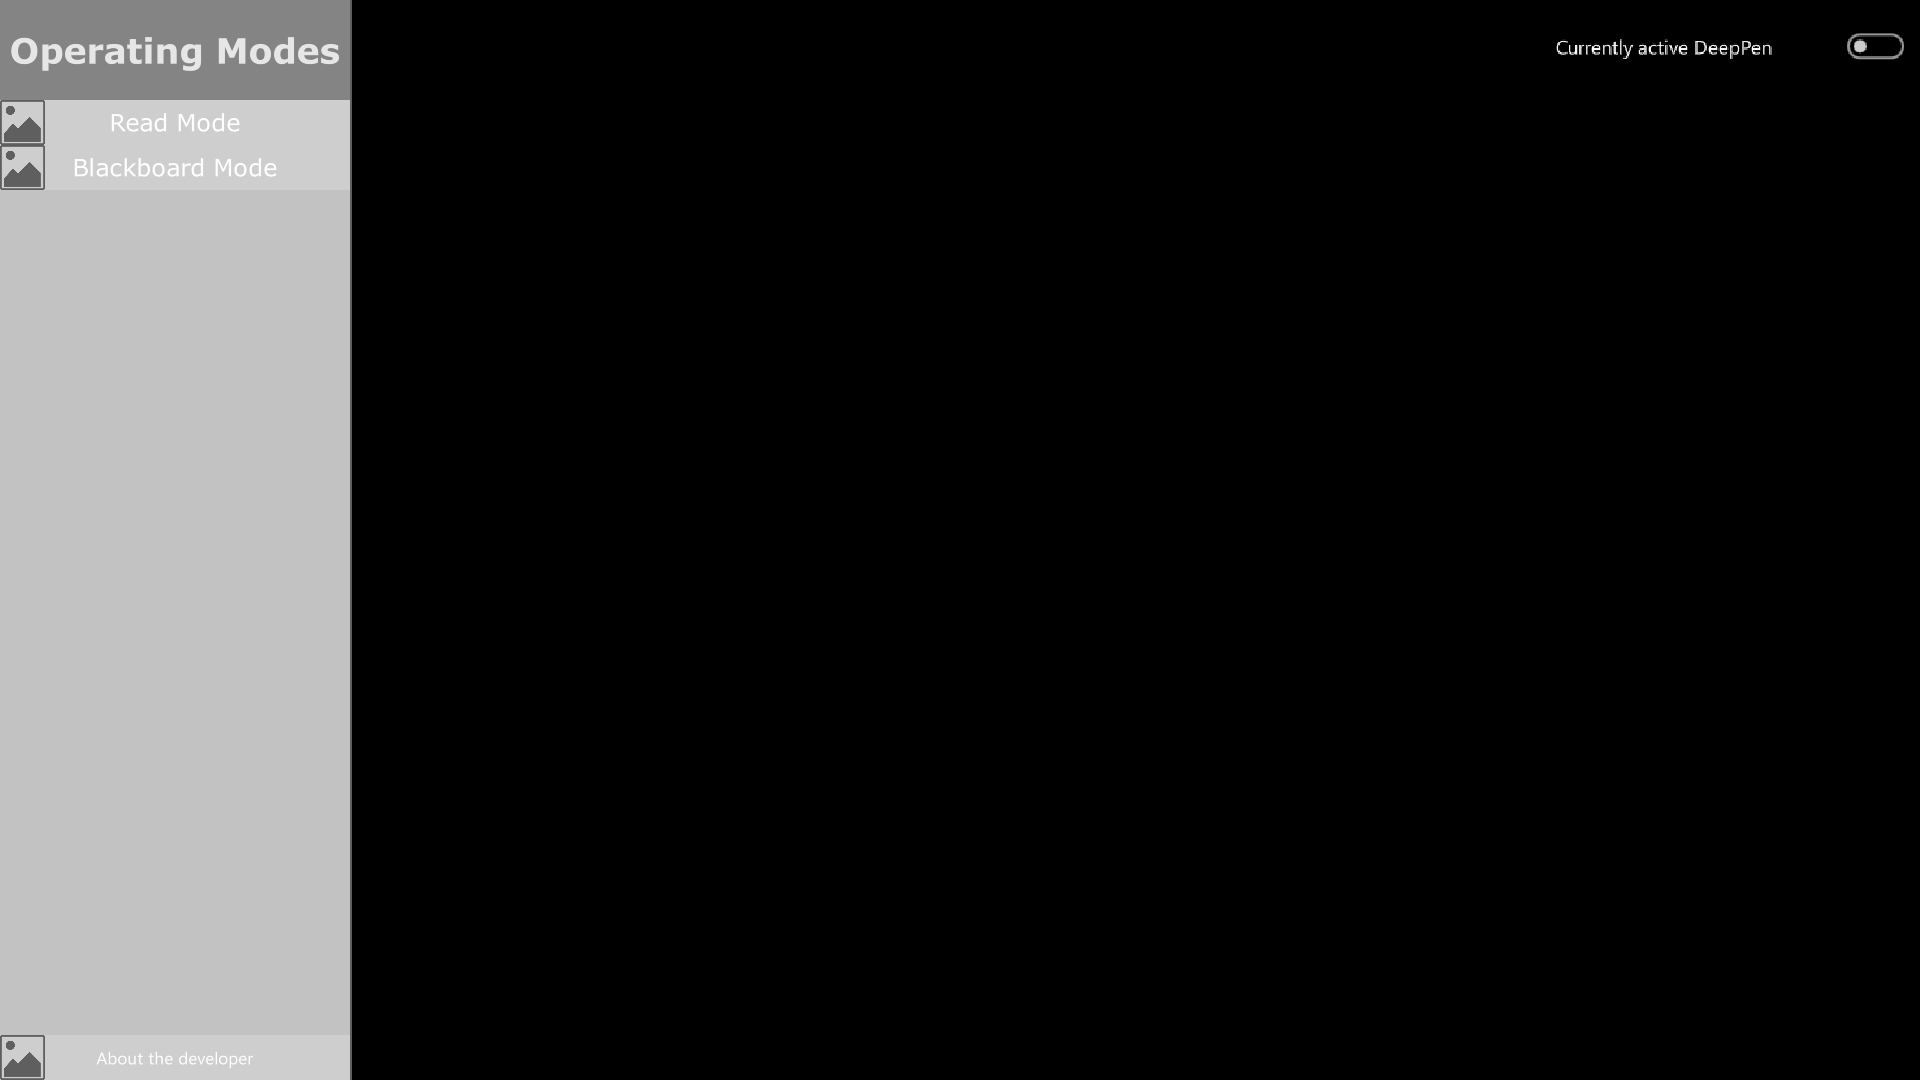
\includegraphics[width=1\textwidth]{capturas/DisenoUsuario1.png}\\[-0,40cm]
    \caption{Primer boceto en QT Design Studio}
    \end{figure}

Con este primer acercamiento, dispuse los elementos que pensé imprescindibles.
No obstante, al finalizar esta primera iteración de diseño, pude ver que las
carencias a nivel estético; facilmente resolubles cuando comience con la
implementación real en \textbf{\textit{QT Creator}}. También vi que faltaban
algunos botones como el de sincronización con el \textbf{\textit{DeepPen}},
que \textit{Read Mode} no era un buen nombre para indicar el comportamiento
del modo, o que había un espacio en el centro de la barra superior sin usar y
que podía usar para indicar el modo actual.

\pagebreak

Teniendo estas apreciaciones en mente, las corregí en la siguiente iteración
de aproximación al diseño con el que partir en la implementación.

\begin{figure}[h]
    \centering
    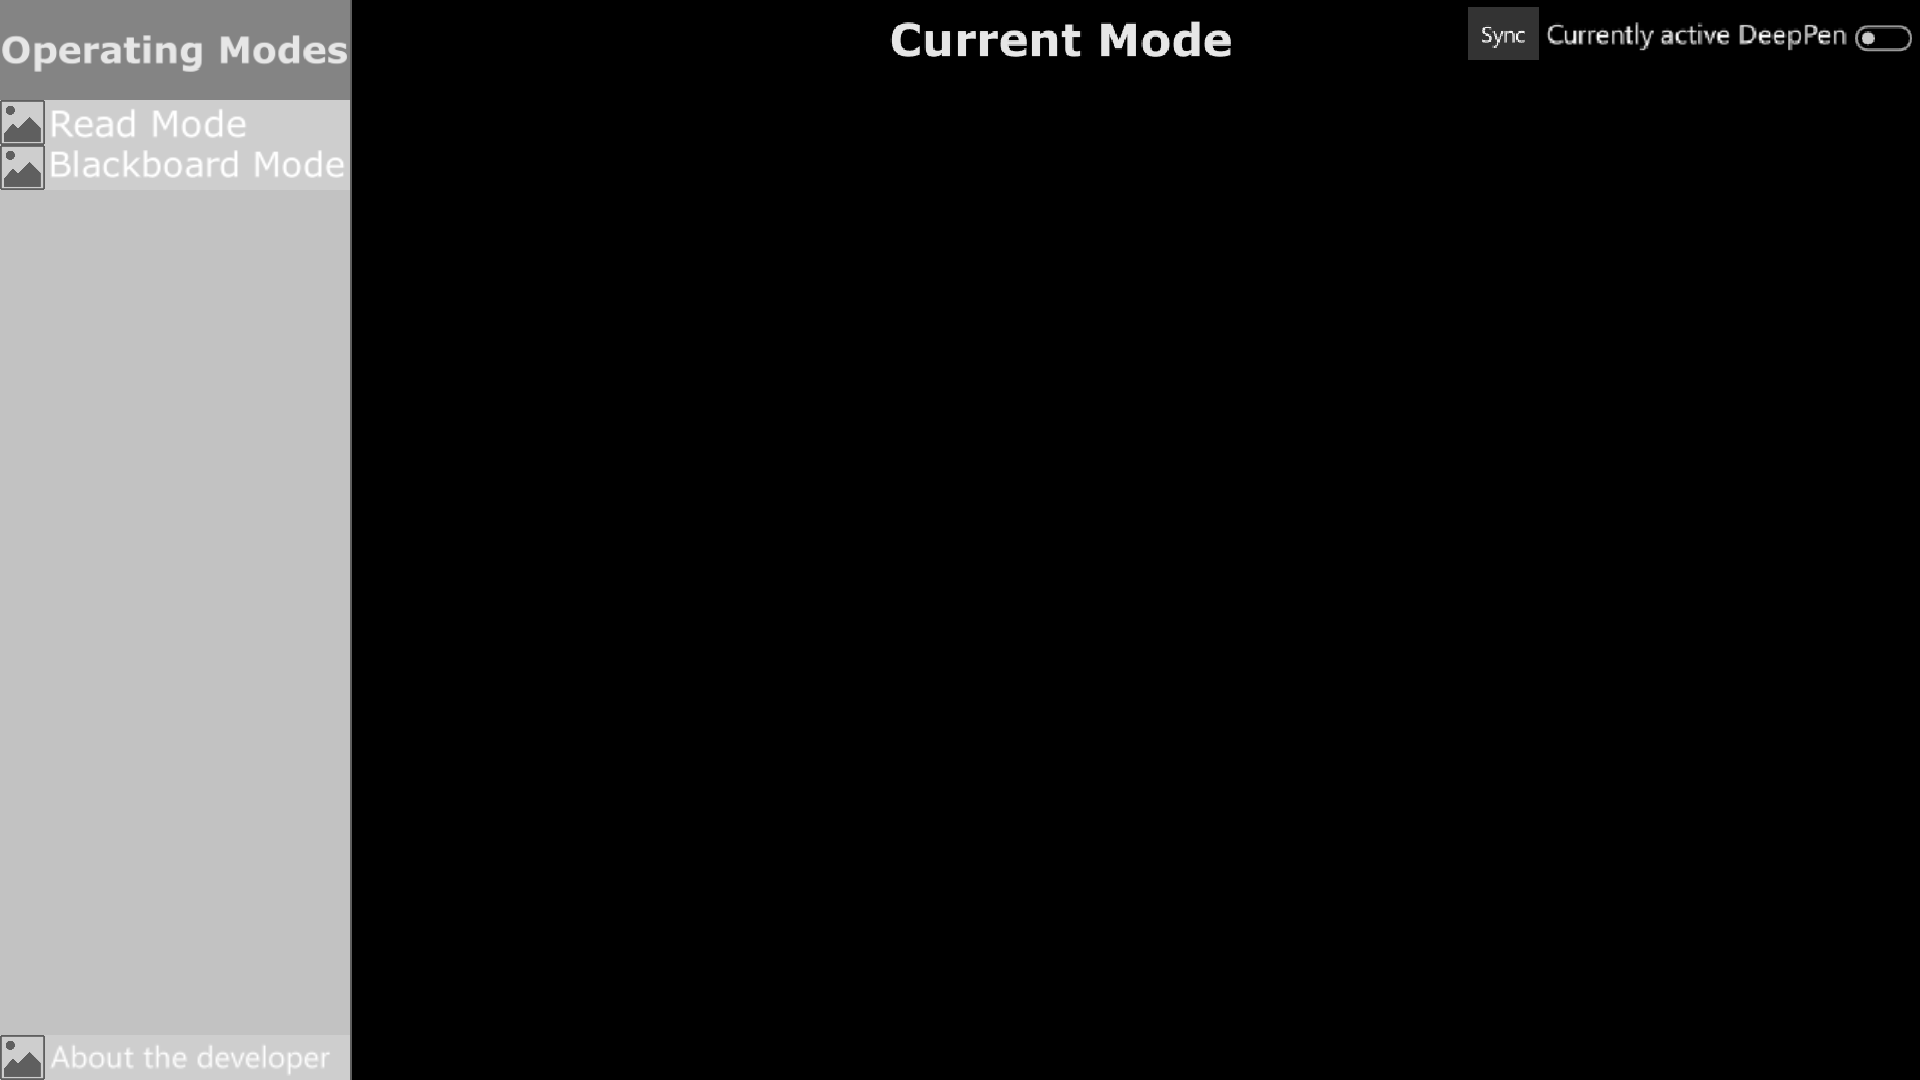
\includegraphics[width=1\textwidth]{capturas/DisenoUsuario2.png}\\[-0,40cm]
    \caption{Segundo boceto en QT Design Studio}
    \end{figure}

Para pasar esta aproximación de diseño a una implementación real, utilicé
\textbf{\textit{QT Creator}} con \textbf{\textit{C++}}. Resultando en lo siguiente:

\begin{figure}[h]
    \centering
    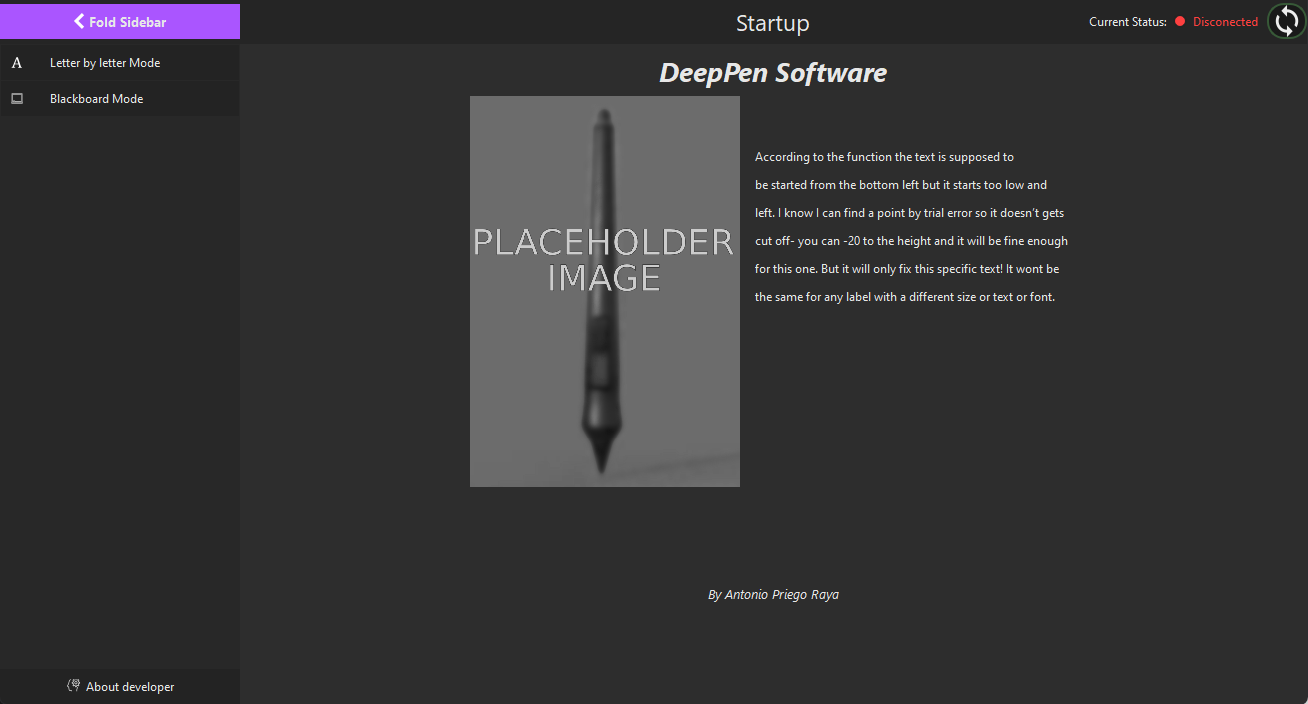
\includegraphics[width=1\textwidth]{capturas/Interfaz.png}\\[-0,40cm]
    \caption{Primera implementación de la interfaz de usuario del
    \textbf{\textit{DeepPen}}}
    \end{figure}



	% Entrenamiento
	\begin{mimargen}{-0.65cm}{-1cm}
\chapter{Entrenamiento}

Para comenzar con Arduino+TensorFlow, instalaré la bibliotecas
necesarias para usar TensorFlow y la \textit{Nano 33 Sense}:
\begin{enumerate}
    \item \textbf{Arduino\_TensorFlowLite}: Permite construir aplicaciones con
    aplicaciones para AI/ML.
    \item \textbf{Arduino\_LSM9DS1}: Provee de las herramientas para acceder al
    acelerómetro, magnetometro y giroscopop del \textit{Nano 33 BLE Sense}.
\end{enumerate}

\cite{github-magicwand}Además, hay que realizar una serie de cambios en la biblioteca
\small\textbf{LSM9DS1.cpp}.\normalsize\\
Añadir justo antes de que la función \small\textbf{LSM9DS1Class::begin()}\normalsize
~retorne:
\begin{lstlisting}
    // Enable FIFO (see docs https://www.st.com/resource/en/datasheet/DM00103319.pdf)
    writeRegister(LSM9DS1_ADDRESS, 0x23, 0x02);
    // Set continuous mode
    writeRegister(LSM9DS1_ADDRESS, 0x2E, 0xC0);
\end{lstlisting}

También debemos editar \small\textbf{LSM9DS1Class::accelerationAvailable()}
\normalsize:
\begin{lstlisting}
    int LSM9DS1Class::accelerationAvailable()
    {
        /********************************** OLD *********************************
        if (readRegister(LSM9DS1_ADDRESS, LSM9DS1_STATUS_REG) & 0x01) { 
            return 1; 
        }
        *********************************** OLD *********************************/
    
        // Read FIFO_SRC. If any of the rightmost 8 bits have a value, there is data
        if (readRegister(LSM9DS1_ADDRESS, 0x2F) & 63) {
            return 1;
        }
        
        return 0;
    }
\end{lstlisting}

Si queremos acceder al puerto serie de la placa o usar el IDE de Arduino, debemos
conceder permisos al dispositivo:
\begin{lstlisting}[language=bash]
    ~$ ls -l /dev/ttyACM*                     # En mi caso
    ~$ sudo usermod -a -G dialout <usuario>
\end{lstlisting}~\\


Cuando ya tenemos la biblioteca para los sensores y el acceso al puerto garantizado,
podemos pasar a probar el programa.
Si funciona con el entrenamiento por defecto, continuamos finalmente con nuestro
entrenamiento.\\
Realizaremos el entrenamiento recogiendo muestras para cada caracter a
reconocer. Una vez tenemos suficientes muestras para todos los caracteres, podemos
realizar el entrenamiento del modelo, que realizaremos en \textit{Google Colab}.
El script de entrenamiento es el siguiente: [\textbf{METER ENLACE}].

~\\
Toma de muestras, para el software que utilizaremos para tomar los datos
para crear el dataset con el que entrenar el modelo, necesitaremos instalar las
siguientes bibliotecas:\\
\cite{apds9960} Arduino\_APDS9960: para disponer de librerías para algunos sensores adicionales.\\
\cite{cmsisdsp} Arduino\_CMSIS\-DSP: para disponer de arm\_math.h.\\
\cite{lps22hb} Arduino\_LPS22HB: herramientas para disponer del sensor de presión.\\
\cite{hts221} Arduino\_HTS221: herramientas para el sensor de temperatura y humedad.

\end{mimargen}

	% Notas
	\begin{mimargen}{-1cm}{-1cm}

\chapter{Apéndice}

\section{Problemas técnicos}

\subsection{Si la placa deja de ser detectada}
En la primera subida del programa con los datos de entrenamiento
creados por mí, la placa dejó de ser detectada por el ordenador.\\
Lo cual me llevó a pensar que el bootloader se había corrompido.
Sin embargo, buscando posibles causas, encontré una solución:
restaurar manualmente la placa, cosa que solo funciona, evidentemente,
si el bootloader no está dañado.
Pulsando el botón reset de la placa rápidamente varias veces justo
al conectarlo al ordenador, puede restaurarse la placa. Si ha funcionado,
el "L" led se encenderá.

Esto ocurría al incorporar el modelo de datos que yo mismo entrenaba
y fue uno de los problemas que más tiempo me llevó solucionar, sobre
todo porque no tenía ningún tipo de referencia de por qué no estaba
respondiendo correctamente el programa con el nuevo modelo.\\
Por suerte llegué a la solución:\\~\\


\subsection{El modelo de datos entrenado no responde\cite{intro-tensor-micro}}
Como explico en caso anterior, la incorporar el modelo de datos
entrenado con el dataset de ejemplo que proporciona TensorFlow,
al subir el programa a la placa, esta dejaba de reconocerse por
el ordenador, teniendo que resetear la flash de la placa.\\
Esto se debía a que el proyecto Arduino no soportaba una de las
operaciones que realiza nuestro modelo(reshape).\\
\newpage Podemos solucionar esto de dos formas:
\begin{enumerate}
    \item (No probada) Simplemente hacer uso de AllOpsResolver,
    de forma que el interprete tendrá acceso a todas las operaciones
    disponibles.
    \item Esta segunda es la más sofisticada, ya que al no disponer
    de todas las operaciones para el interprete, reduciremos la cantidad
    de memoria que ocupamos.\\Es la que yo implementé.
\end{enumerate}

Añadir la siguiente línea al archivo \small\textbf{*.ino}\normalsize~
de nuestro proyecto:
\begin{lstlisting}
micro_mutable_op_resolver.AddBuiltin(tflite::BuiltinOperator_RESHAPE,
                                      tflite::ops::micro::Register_RESHAPE());
\end{lstlisting}

De esta forma estamos añadiendo la operación al repertorio de las que tendrá
disponibles el interprete\small\textit{(static\_interpreter)}\normalsize,
\small\textbf{micro\_mutable\_op\_resolver}\normalsize.

\begin{figure}[h]
\begin{lstlisting}[firstnumber=72]
static tflite::MicroMutableOpResolver micro_mutable_op_resolver;  // NOLINT
micro_mutable_op_resolver.AddBuiltin(
    tflite::BuiltinOperator_DEPTHWISE_CONV_2D,
    tflite::ops::micro::Register_DEPTHWISE_CONV_2D());
micro_mutable_op_resolver.AddBuiltin(
    tflite::BuiltinOperator_MAX_POOL_2D,
    tflite::ops::micro::Register_MAX_POOL_2D());
micro_mutable_op_resolver.AddBuiltin(tflite::BuiltinOperator_CONV_2D,
                                     tflite::ops::micro::Register_CONV_2D());
micro_mutable_op_resolver.AddBuiltin(
    tflite::BuiltinOperator_FULLY_CONNECTED,
    tflite::ops::micro::Register_FULLY_CONNECTED());
micro_mutable_op_resolver.AddBuiltin(tflite::BuiltinOperator_SOFTMAX,
                                     tflite::ops::micro::Register_SOFTMAX());
micro_mutable_op_resolver.AddBuiltin(tflite::BuiltinOperator_RESHAPE,
                                     tflite::ops::micro::Register_RESHAPE());
                                     
// Build an interpreter to run the model with
static tflite::MicroInterpreter static_interpreter(
    model, micro_mutable_op_resolver, tensor_arena, kTensorArenaSize,
    error_reporter);
interpreter = &static_interpreter;
\end{lstlisting}
\caption{Fragmento de \small\textbf{*.ino}\normalsize~ de nuestro proyecto.}
\end{figure}

Este fragmento de código ilustra lo que acabo de explicar.


\subsection{Error durante el entrenamiento}
Al comenzar con mi primer pequeño dataset para comprobar cuán realizable es
mi idea para este modelo, tuve un error que me tuvo durante un buen tiempo
ocupado.

\begin{figure}[h]
    \centering
    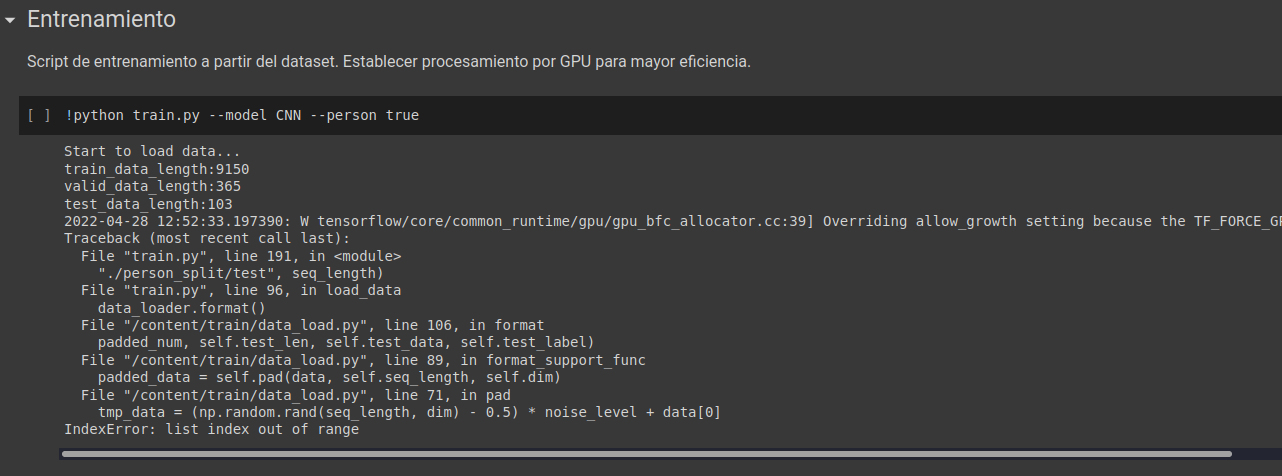
\includegraphics[width=1\textwidth]{capturas/ErrorEntrenamiento.png}\\[-0,40cm]
    \caption{Error durante primer entrenamiento con un dataset propio.}
    \end{figure}

Tras revisar que no se debía a la longitud de las secuencias de datos,
como hace pensar el mensaje de error, fui a intentar reducir el tamaño de las
muestras del dataset y fue cuando vi que había un error en una de las muestras,
de forma que había un separador (' -,-,-') sin información.\\
Al eliminarlo, el entrenamiento ya no arrojaba errores.


\subsection{Error al cambiar el tamaño de las secuencias de movimientos}
Los movimientos que se deben registrar para las letras son, en general, más complejos
que los que incluye el dataset de ejemplo. Por lo tanto las secuencias de registro
de movimiento, serán mayores. Esto supone un problema porque el modelo está ajustado
al dataset de ejemplo y por tanto, se queda algo corto para nuestro propósito.
El error se da al cambiar el tamaño de dicha secuencia
(\small\textbf{seq\_length}\normalsize) en \small\textbf{train.py}\normalsize~ y
\small\textbf{train\_test.py}\normalsize~.

\begin{figure}[h]
    \centering
    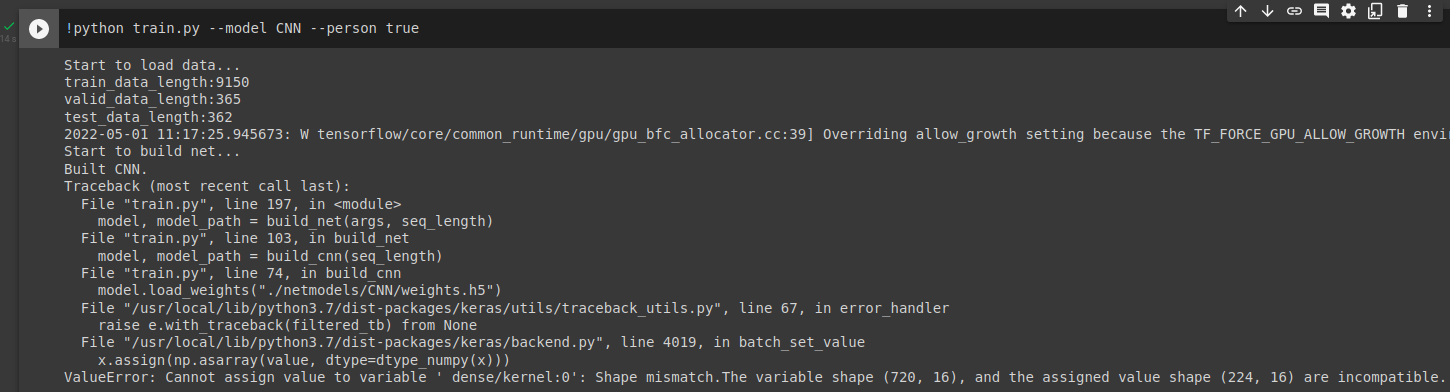
\includegraphics[width=1\textwidth]{capturas/ErrorTamanioSecuencias.png}\\[-0,40cm]
    \caption{Error al cambiar el tamaño de secuencia de movimientos.}
    \end{figure}

Tras mucha documentación sobre Tensorflow, y no obtener la causa del error; pensé
que esto ya me pasó por culpa de la configuración del \small\textbf{*.ino}\normalsize~.
Así que fui a revisarlo y efectivamente, hay un parámetro en este archivo sujeto a
la longitud de los datos. Tras cambiarlo, funcionaba correctamente de nuevo, aunque
sin detectar la letra que estaba probando en el nuevo dataset.


\subsection{Valores nulos al leer por Bluetooth QT}
Tras mucho tiempo implementando e intentando dar con el error de por qué no se
leía ninguna characteristic del dispositivo pese a estar detectándolas y estar
correctamente conectado, se debía a dos factores.\\
El primero estar haciendo uso de una librería anterior a la documentación con
la que estaba trabajando(Librería de QLowEnergyService). Hay grandes diferencias
en el comportamiento de algunos métodos de esta librería de las versiones 5.x
a la 6.x, aunque por desgracia, estas no provocan errores, hacen que el
el código no funcione como se esperaría(Enums con valores diferentes o inexistentes, etc).\\
En segundo lugar estaba llamando a un método cuando todavía no se había recibido
la characteristic. Por tanto esta aparentaba estar bien registrada, ya que
podía obtener su Uuid, pero no contenía ningún valor.
Estaba leyendo en connectToService() y no en serviceDetailsDiscovered().\\

He instalado  ArduinoBLE.h para probar sketch de harvard\\
\url{https://create.arduino.cc/projecthub/sibo_gao/harry-potter-magic-wand-384477}


Orientación para vTensorFlow no Harvard:
\url{https://github.com/andriyadi/MagicWand-TFLite-Arduino/blob/master/src/accelerometer_handler.cpp}


Para modo pizarra:
\url{https://github.com/petewarden/magic_wand/blob/main/website/index.html}.
\url{https://tinyml.seas.harvard.edu/magic_wand/}


\end{mimargen}

	% Notas
	\begin{mimargen}{-1cm}{-1cm}

\chapter{Intento Harvard}

Comienzo ejecutando tal cual el código del repo
\url{https://github.com/petewarden/magic_wand}.

Importante tener la biblioteca de tensorflow actualizada(en este
caso la provista por pete warden).

Visto cómo toma pete los datos, pruebo a hacerlo.
Cargar el programa de recolección de datos en la placa(creo que funciona el magic\_wand,
PROBAR).
Acceder a la web de recolección. Recolectar.
Para acceder a la web, hay que hacerlo con chrome y con la flag
'Experimental Web Platform features' activa en 'chrome://flags/'


Hay un error con el DataCollector, además de que asigna mal los índices(index)
al borrar muestras, no guarda todas las muestras que tomas, da la sensación de que
hay un límite.
Para contar el número de muestras que hay en el JSON, uso la siguiente línea bash:
\begin{lstlisting}[language=bash]
~$ grep -o index <nombre_archivo>.json | wc -l
\end{lstlisting}



\textbf{CAMBIAR ORIENTACIÓN DE LA PLACA} \\
Como no hay referencias de la orientación original de los sensores en ningún
datasheet, con el propio sketch que hice originalmente para tomar las muestras,
comprobé la posición con la que funciona, la comparé con la posición que quiero
tener y gracias a eso pude hacer el siguiente cambio.\\
Lo mejor que he conseguido cambiando en la biblioteca de los sensores,
en LSM9DS1.cpp en todas los sensores:
\begin{lstlisting}[language=c++]
//          Original         //     Orientacion cambiada
x = data[0] * 4.0 / 32768.0; // z = -data[0] * 4.0 / 32768.0;
y = data[1] * 4.0 / 32768.0; // y =  data[1] * 4.0 / 32768.0;
z = data[2] * 4.0 / 32768.0; // x =  data[2] * 4.0 / 32768.0;
\end{lstlisting}

\newpage
Creo que habría que cambiar algo de deep\_pen.ino(a partir de línea 408)
\begin{lstlisting}[language=c++]
    const float gy = current_gravity[1];
    const float gz = current_gravity[2];
    float gmag = sqrtf((gy * gy) + (gz * gz));
    if (gmag < 0.0001f) {
      gmag = 0.0001f;
    }
    // ...
\end{lstlisting}


\textbf{LA OBTENCIÓN DE DATOS TIENE UN FALLO AL BORRAR MUESTRAS} \\
Este fallo aparentemente se produce al borrar instancias por debajo de
la última. En ocasiones, se produce un pequeño error en las comprobaciones
de índices de muestras, por lo que se borran varias muestras y estas terminan
con índices desordenados.\\
Para paliar este problema, he creado un pequeño script que toma el número de
muestras y ordena los índices de las mismas.\\

\textbf{MODELO}\\
Se trata de un modelo de aprendizaje supervisado, es decir, que está basado en
etiquetas(\textit{labels}) estas etiquetas representarán las distintas soluciones
a las que hará frente el modelo; en nuestro caso, letras.
La forma que emplearemos para representar dichas letras como input para el modelo,
serán imágenes. Aunque para tomar dichas imágenes, hacemos uso del giroscopio
y el acelerómetro de la placa.\\


\textbf{LEER DEL PUERTO SERIE EN QT}
Hay que añadir al *.pro del proyecto QT:
\begin{lstlisting}[language=make]
  QT += serialport
\end{lstlisting}
Y tras esto, añadir la biblioteca con normalidad y acceder al puerto
con el nombre, en nuestro caso, "ttyACM0".\\\\

\textbf{FALLO RECONOCIMIENTO DE IMÁGENES QT}\\
Al importar imágenes en QT tras haber exportado el programa a Win y Linux para
probar que todo fuera correctamente, las imágenes dejaron de mostrarse.\\
Esto se debe a que cambió la ruta del proyecto al directorio en el que se
exportó. Por tanto las rutas especificadas para las imágenes, dejaron de ser
válidas. Para corregir este problema, basta con cambiar el 'Build directory' del
proyecto(Desde 'Projects' en el panel de la derecha del QT creator).\\

\textbf{HEBRAS QT}\\
Para la lectura del puerto serie desde el programa, necesitamos imporat

\textbf{VISOR WEB QT}\\
Para hacer empotrar html en qt, importamos las bibliotecas de QWeb. Para ello,
necesitamos aantes instlar todo el QtWebKit siguiendo las instrucciones:
\url{https://github.com/OpenBoard-org/OpenBoard/wiki/Build-OpenBoard-on-Ubuntu-20.04}

\textbf{VINCULAR PUERTO SERIE A PLACA}\\
Para ello, haré uso de las reglas de udev del sistema linux.
Lo primero es conocer la información de nuestra placa:
\begin{lstlisting}[language=make]
  ~$ lsusb
[...]
Bus 003 Device 004: ID 2341:805a Arduino SA Nano 33 BLE
[...]
\end{lstlisting}
De aquí podemos extraer el fabricante(o idVendor) y el producto de este fabricante
(o idProduct). Necesitaremos ambos.

Ahora necesitamos el serial del puerto al que vincularemos la placa:
\begin{lstlisting}[language=make]
  ~$ udevadm info -a -n /dev/ttyACM0 | grep serial
ATTRS{serial}=="185F25FD3EF48040"
\end{lstlisting}
Con esto, ya podemos crear la regla para vincular univocamente el puerto a la placa
y evitar así problemas con la detección en el UI.\\
En /etc/udev/rules.d/99-ftdi.rules (en mi caso, varía dependiendo del sistema),
crearemos la regla \\SUBSYSTEM=="tty", ATTRS{idVendor}=="2341", ATTRS{idProduct}=="805a",
ATTRS{serial}=="185F25FD3EF48040", SYMLINK+="ttySLAB0"\\por los datos obtenidos.\\

\textbf{CAMBIOS MODELO}\\
Cambiar el tamaño del kernel de las capas Conv2D de 3 a 4, resulta muy efectivo,
a costa, evidentemente, de aumentar el tamaño que ocupa el modelo.\\
Al pasar de 4 a 5, el modelo arroja unos datos de efectividad teóricos extremadamente
buenos, alcanzando cifras de precisión mucho más altas con menos epochs.
En general, podemos extrapolar que, a mayor tamaño del kernel, mejor precisión pero
mayor tamaño del modelo. En nuestro caso no llega a ser un problema, ya que, aunque
estamos usando un dispositivo de memoria limitada, no llega a ocuparse toda la memoria
del mismo, al menos por ahora.\\

\textbf{PRUEBAS BLUETOOTH}\\
He tenido que instalar qtconnectivity5-dev para probar el QT project que estoy probando.\\

\textbf{POR QUÉ ESTA PLACA?}\\
Aduino Nano Sense 33 BLE\\
Por qué arduino: Documentación, respaldo comunidad, IDE facilita trabajo, etc.\\
Por qué Nano: Queremos integrarla en un 'lápiz', debe ser un dispositivo pequeño.\\
Por qué Sense: Necesitamos los sensores para el reconocimiento de movimiento.\\
BLE: Por pura utilidad, es mucho más cómodo utilizar el lápiz de forma inalámbrica.
Además no tiene mucho sentido integrar el procesamiento en un dispositivo pequeño
si va a depender de un ordenador.\\

\textbf{DESCONEXIÓN DEL PROGRAMA A BT AL ESCRIBIR PLACA EN RX}\\
Para el control de flujo de la comunicación bluetooth(asegurarse de que recibimos
bien y solo una vez cada letra), implemento un sistema de señales.
Cuando recibimos una letra desde la placa(mediante canal tx), el programa la almacena y
envía una señal de que ha recibido la letra(mediante canal rx) y cuando la placa
recibe esta señal, borra del canal tx la letra para que no vuelva a leerse desde el
programa.
El problema descrito, viene, creo, al escribir en rx la señal de recibo. Por algún
motivo, el programa se desconecta de la placa.\\


\textbf{MÉTODO DE ENVÍO DE BUFFER DE LETRAS PARA CONEXIÓN BT CUANDO HAYA UNA CADENA
PREVIA A CONEXIÓN}\\

~\\~\\~\\Documentación Bluetooth LE:
https://doc.qt.io/qt-6/qtbluetooth-le-overview.html

~\\~\\~\\Visualizar red neuronal :
http://alexlenail.me/NN-SVG/index.html

~\\~\\~\\Documentación sobre Keras:
https://keras.io/api/

\end{mimargen}

	% Herramientas
	\chapter{Herramientas}

\begin{mimargen}{-0.5cm}{-1.8cm}

        
    \begin{enumerate}
        \item \textbf{QT Designer}({\tiny Licencia de Codigo Abierto}):
        Bocetado de la interfaz de usuario.
        \item \textbf{QT Creator}({\tiny Licencia de Codigo Abierto}):
        Implementación de la interfaz de usuario.\\
        (v6.2.4-Linux | v6.2.2-Windows)
        \item \textbf{Arduino IDE}: Desarrollo del software para el DeepPen.
        \item \textbf{Visual Studio Code + Latex}: Creación de la memoria.
        \item \textbf{Bibliotecas}:
        \subitem TensorFlowLite(Arduino).
        \subitem Arduino\_LSM9DS1(Arduino).
        \subitem libglu1-mesa-dev (Para QT linux).
    \end{enumerate}



\end{mimargen}

	% Introducción 
	\chapter{Introducción}

Este proyecto es software libre, y está liberado con la licencia \cite{gplv3}.

	% Descripción del problema y hasta donde se llega
	\chapter{Descripción del problema}


	
	\chapter{Planificación}

\section{Metodología utilizada}


\section{Temporización}

\section{Seguimiento del desarrollo}


	% Análisis del problema
	% 1. Análisis de requisitos
	% 2. Análisis de las soluciones
	% 3. Solucion propuesta
	% 4. Análisis de seguridad
	\chapter{Análisis del problema}
 


	% Desarrollo bajo sprints: 
	% 	1. Permitir registros y login de usuarios
	% 	2. Desarrollo del sistema de incidencias
	% 	3. Desarrollo del sistema de denuncias administrativas y accidentes
	% 	4. Desarrollo del sistema de croquis
	%   5. Instalación de la aplicación de manera automática
	\chapter{Implementación}

La implementación del software se ha dividido en hitos. Estos, han sido definidos en Github
y cada uno de ellos contiene un grupo de \textit{issues} que se corresponden con las distintas
mejoras que se han ido incorporando al software a lo largo de su desarrollo.\\



	% Presupuesto

	% Conclusiones
	\chapter{Conclusiones y trabajos futuros}



	% Trabajos futuros


	\newpage
	\bibliography{bibliografia}
	\bibliographystyle{plain}
	
\end{document}

